\documentclass{beamer}
\usepackage[utf8]{inputenc}
\usepackage[T1]{fontenc}
\usepackage{lmodern}
\usepackage[ngerman]{babel}
\usepackage{graphicx}
\usepackage{listings}
\usepackage{verbatim} % mainly for multi-line comments

%\usetheme{Madrid}
%\useinnertheme{rectangles}
%\setbeamertemplate{navigation symbols}{}
\setbeamercovered{highly dynamic}

\title{Tracking juggling balls using the Kinect}
\subtitle{final presentation}
\author[Rolf $\cdot$ Thiemo $\cdot$ Flo]{Rolf Boomgaarden $\cdot$ Thiemo Gries $\cdot$ Florian Letsch}
\institute{Universität Hamburg}
\date{19/12/2013}

\begin{document}

\frame
{
\titlepage
}
\section{Looking back}

\section{Our plan}
\begin{frame}{What we thought at first}
\begin{center}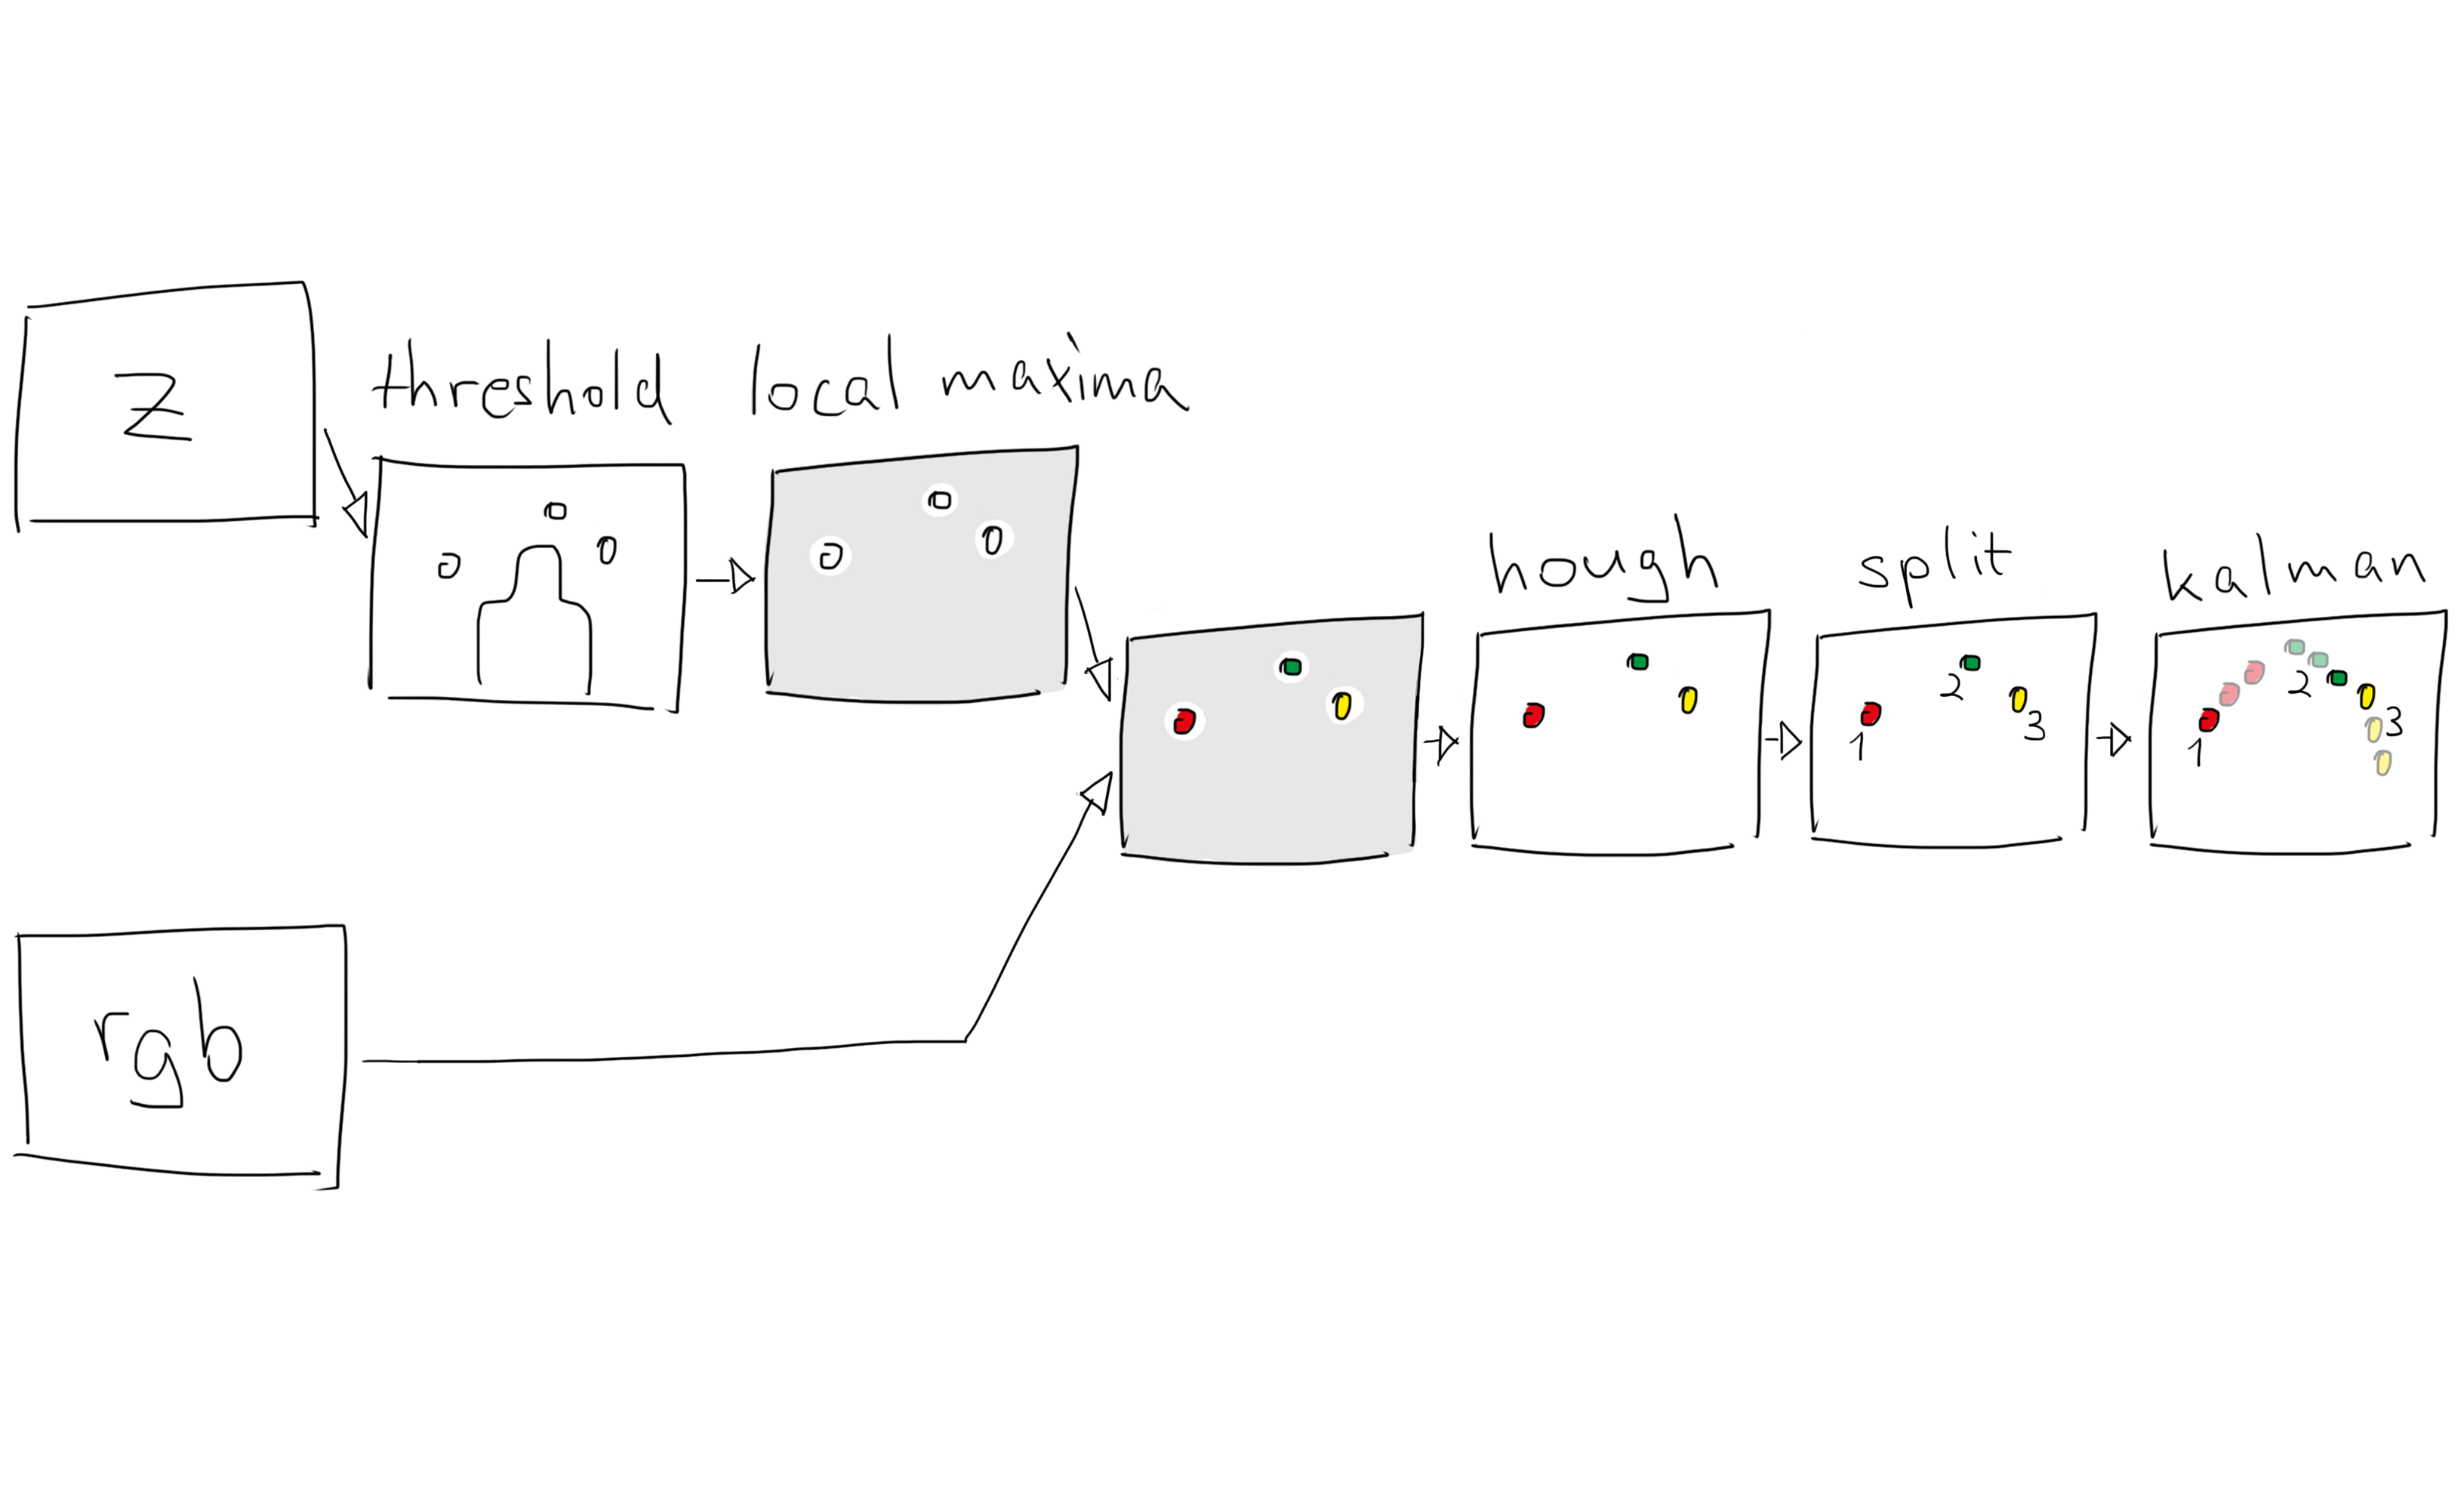
\includegraphics[scale=0.1]{img/flowchart.png}\end{center}
\end{frame}

\begin{frame}{A \textit{"working"} solution}
\begin{enumerate}
	\item detection with depth data (no rgb)
	\item cut off depth at threshold ($\rightarrow$ binary representation)
	\item find bounding rects (\lstinline{OpenCV.BoundingRect})
	\item filter out small rectangles and rectangles touching the image boundaries
	\item find centroid of remaining rects. The three rects closest to centroid are considered "balls"
	\item a ball fits inside a rectangle (close representation of actual ball in RGB, ignoring the deformation caused by movement)
\end{enumerate}
\end{frame}


\begin{frame}{A checklist}
WORKS:

\begin{itemize}
\item Using dummy data (numpy array dumps)\\
\item Use a hard coded threshold\\
\item filter out rectangles too small or too close to image edge
\end{itemize}

DOESN'T REALLY WORK:

\begin{itemize}
 \item Match balls from frame to frame
\end{itemize}

NOT THERE YET:
\begin{itemize}
 \item Kalman filter
\end{itemize}

\end{frame}



\begin{frame}{Challenges}
\begin{itemize}
	\item Local maxima
	\item Multiple balls (colour?)
\end{itemize}
\end{frame}

\begin{frame}{The end}
EOF
\end{frame}

\end{document}






